\documentclass[tikz,border=8pt]{standalone}
% Shared look for every TikZ diagram. Load with \input{../../tools/tikz-style.tex}
\usepackage[T1]{fontenc}
\usepackage{lmodern}
\renewcommand{\sfdefault}{lmr}  % diagrams use the same serif as the text
\usetikzlibrary{arrows.meta, positioning, shapes.geometric, calc, fit, backgrounds}
\definecolor{cblue}{HTML}{4C78A8}
\definecolor{corange}{HTML}{F58518}
\definecolor{cgreen}{HTML}{54A24B}
\definecolor{cred}{HTML}{E45756}
\definecolor{cpurple}{HTML}{B279A2}
\definecolor{cgrey}{HTML}{6B6B6B}
\tikzset{
  every picture/.style={font=\sffamily, line width=1.2pt},
  box/.style={draw=#1, fill=#1!12, rounded corners=4pt, align=center, inner sep=7pt, minimum height=1.1cm},
  box/.default=cgrey,
  arrow/.style={-{Stealth[length=3mm]}, draw=cgrey, line width=1.4pt},
  title/.style={font=\sffamily\bfseries\Large},
  note/.style={font=\sffamily\small, text=cgrey, align=center},
}
\AtBeginDocument{\hyphenpenalty=10000 \exhyphenpenalty=10000}

\begin{document}
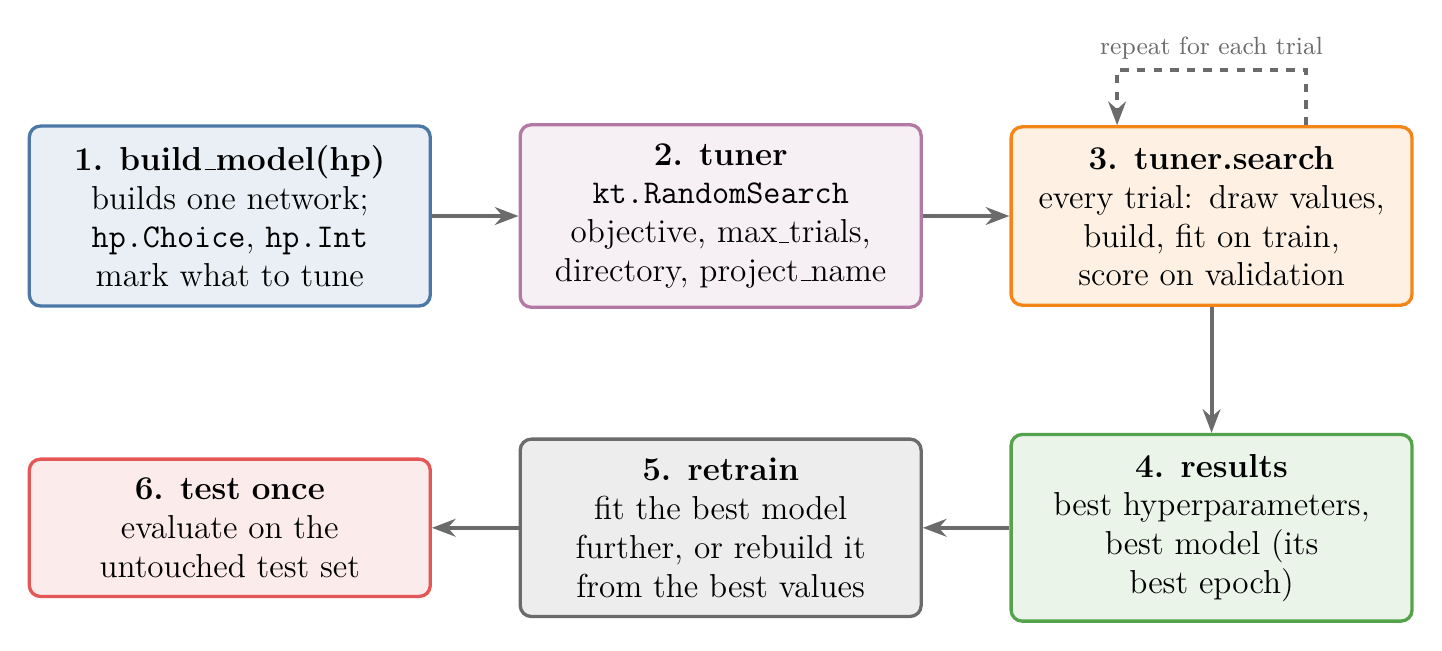
\begin{tikzpicture}[node distance=1.1cm, every node/.append style={font=\sffamily\large}]
  \node[box=cblue, text width=4.6cm] (b) {\textbf{1. build\_model(hp)}\\builds one network;\\\texttt{hp.Choice}, \texttt{hp.Int}\\mark what to tune};
  \node[box=cpurple, text width=4.6cm, right=of b] (t) {\textbf{2. tuner}\\\texttt{kt.RandomSearch}\\objective, max\_trials,\\directory, project\_name};
  \node[box=corange, text width=4.6cm, right=of t] (s) {\textbf{3. tuner.search}\\every trial: draw values,\\build, fit on train,\\score on validation};
  \node[box=cgreen, text width=4.6cm, below=1.6cm of s] (r) {\textbf{4. results}\\best hyperparameters,\\best model (its best epoch)};
  \node[box=cgrey, text width=4.6cm, left=of r] (f) {\textbf{5. retrain}\\fit the best model\\further, or rebuild it\\from the best values};
  \node[box=cred, text width=4.6cm, left=of f] (e) {\textbf{6. test once}\\evaluate on the\\untouched test set};
  \draw[arrow] (b) -- (t);
  \draw[arrow] (t) -- (s);
  \draw[arrow] (s) -- (r);
  \draw[arrow] (r) -- (f);
  \draw[arrow] (f) -- (e);
  \draw[arrow, dashed] ([xshift=1.2cm]s.north) -- ++(0,0.7) -| node[note, pos=0.25, above] {repeat for each trial} ([xshift=-1.2cm]s.north);
\end{tikzpicture}
\end{document}
